\newpage
\section{Design evolution through scrapped designs}

This section has the objective to show the design process of the final component by the various gripper developments, including photos of the claws and occasionally gripper conformations.

\subsection{Static gripper}

In the first stages of development, the main philosophy for the grasping was defined: given the disparity in dimensions in the joint's two main parts, the gripper must act on the smaller side with a motion similar to the gripping of any type of handle. 
To respect this philosophy, a first claw was implemented as a semi-circular crown $5\text{ mm}$ wide and $50\text{ mm}$ long, aiming to completely envelop the small cylinder of the joint. The tampon was also implemented to solve the weight imbalance between the two sides, but the arm was conceived as a solid metal part, rather than sheet metal. The first claw's form is shown below:

\begin{figure}[H]
	\centering
	\begin{minipage}{0.43\textwidth}
		\centering
		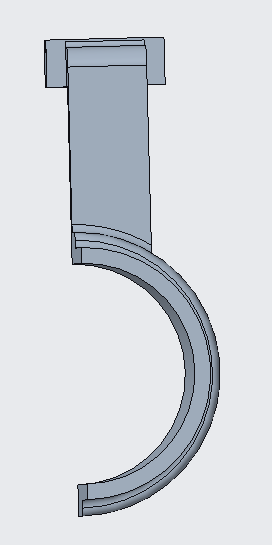
\includegraphics[width=0.5\textwidth]{Immagini/Old models/First claw FW}
		\caption{First claw, front view}
	\end{minipage}
	\hfill
	\begin{minipage}{0.43\textwidth}
		\centering
		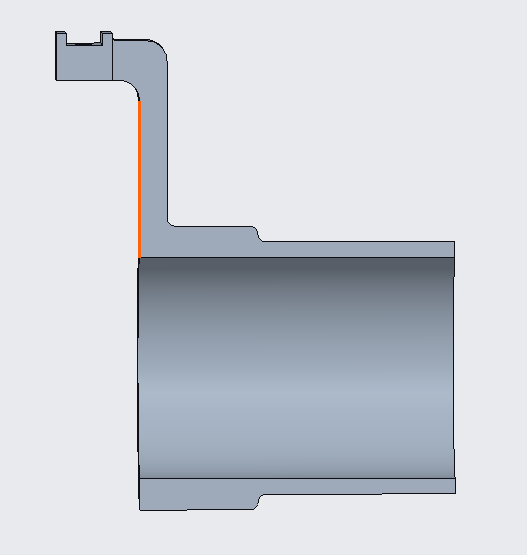
\includegraphics[width=\textwidth]{Immagini/Old models/First claw SW}
		\caption{First claw, side view}
	\end{minipage}
\end{figure}

\begin{figure}[H]
	\centering
	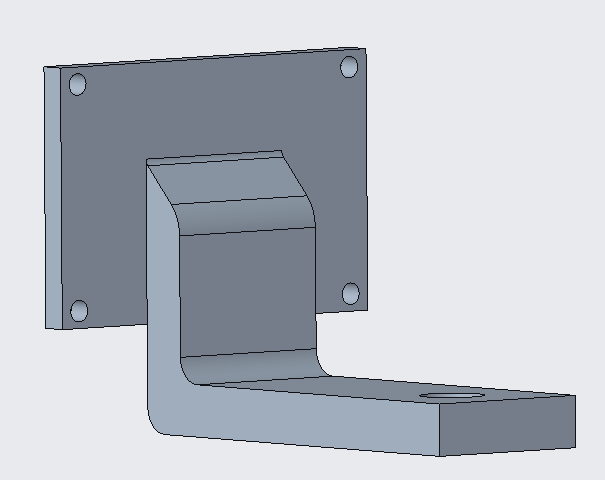
\includegraphics[width=0.5\textwidth]{Immagini/Old models/Braccio}
	\caption{Solid arm}
\end{figure}


Since the joint model used as test subject has a small cylinder circumference of $28\text{ mm}$, this claw was able to grasp it correctly. However, being completely static, the claw was unable to be used in cases where the dimensions would be different than the test radius, which represents an inconvenience in mechanical automated lines.\\
The solid metal arm was also scrapped in favour of a sheet metal structure due to its building complexity in the real world and its negative contribute on weight balancing. 

\subsection{Scrapped arm structures for dynamic claw}

After the failure of the static design, the proposed solution was to use a linkage quadrilateral to let the gripper dynamically reach the component and close itself upon it, following a strict pattern: it is attached on the \texttt{Jodell} component's sliders and moved by those until the proximal link reaches the component; the contact must then force the closing of the quadrilateral around the joint.
This radical change in structure came with tangible challenges and many failed attempts, some of which are reported below: 

\vspace{1cm}
\begin{figure}[H]
	
	\begin{minipage}{0.45\textwidth}
		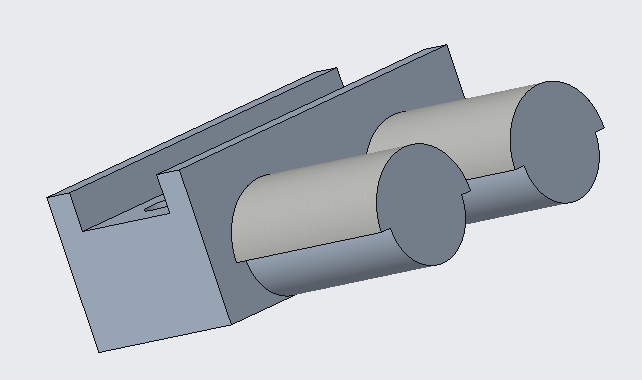
\includegraphics[width=\textwidth]{Immagini/Old models/Base1}
		\caption{Scrapped base for claw}
	\end{minipage}
	\hfill
	\begin{minipage}{0.45\textwidth}
		Here is shown an example of base for a single gripper claw. It uses a $15\times 7\times 6\text{ mm}$ caved block to connect with the \texttt{Jodell}'s sliders and two revolut joints whose exterior is half covered by a $1\text{ mm}$ thick metal coating. This base was scrapped both because the block was too short to actually allow a correct distancing between the two links and because the metal coating on the joints effectively halves the movement freedom for the links. 
	\end{minipage}
	
\end{figure}

\vspace{1cm}

\begin{figure}[H]
	\begin{minipage}{0.35\textwidth}
		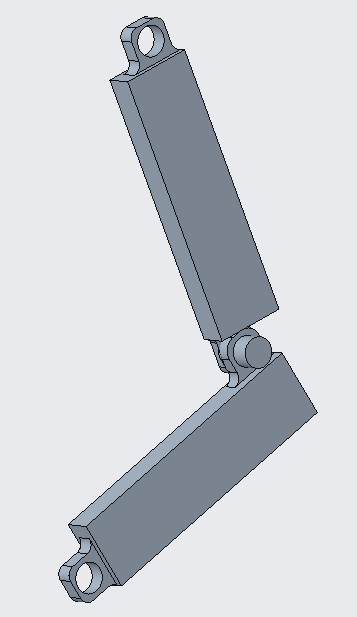
\includegraphics[width=0.9\textwidth]{Immagini/Old models/Arm1}
		\caption{Scrapped model for proximal link}
	\end{minipage}
	\hfill
	\begin{minipage}{0.55\textwidth}
		Here is shown an example of composite proximal link, formed by two solid $3\times 7\times 27\text{ mm}$ links with circle-holed linkages for the revolut joints. The idea was to use the lower link to close on the component when the upper link makes contact with it, but it was scrapped due to several reasons:
		\begin{itemize}
			\item lack of a specific end effector for the gripping;
			\item excessive linkage complexity;
			\item links not thick enough. 
		\end{itemize} 
	\end{minipage}
\end{figure}

\vspace{1cm}
\begin{figure}[H]
	\begin{minipage}{0.37\textwidth}
		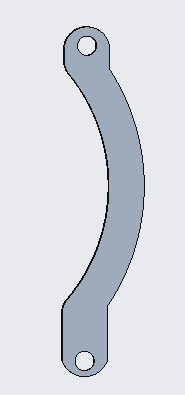
\includegraphics[width=0.6\textwidth]{Immagini/Old models/Arm2}
		\centering
		\caption{Scrapped distal link}
	\end{minipage}
	\hfill
	\begin{minipage}{0.55\textwidth}
		Example of distal link formed with an arch shape between two rounded linkages. Although similar to the final L-shaped distal link, this link was scrapped because of possible collisions with the proximal link when it is moved inwards by the contact with the component. 
	\end{minipage}
\end{figure}

\vspace{1cm}
\begin{figure}[H]
	\begin{minipage}{0.40\textwidth}
		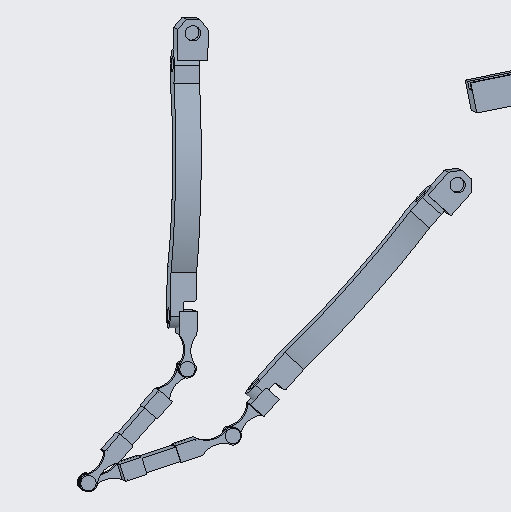
\includegraphics[width=0.8\textwidth]{Immagini/Old models/Gripper1}
		\centering
		\caption{Scrapped claw structure}
		
	\end{minipage}
	\hfill
	\begin{minipage}{0.55\textwidth}
		The claw shown on the left is an example of an embryonal full claw structure formed four straight links and various complex appendages to link them. Despite showing a structure similar to the final one, it was scrapped for problems retained from the component in \texttt{Figure 5}, such as the lack of an end effector and the links being too thin and small. Another issue is caused by the linkages being "jewelry pieces", or pieces too small to be realistically built without loss of resources due to excessive complexity: this pieces were integrated with the links in the final design to form unique pieces that serve all purposes.  
	\end{minipage}
\end{figure}

\vspace{1cm}
\begin{figure}[H]
	
	\begin{minipage}{0.45\textwidth}
		
		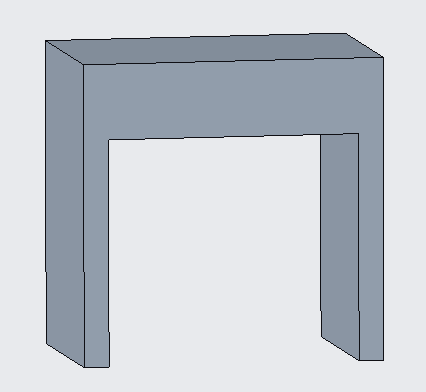
\includegraphics[width=0.8\textwidth]{Immagini/Old models/Anchor}
		\centering
		\caption{Fixed anchor}
	\end{minipage}
	\hfill
	\begin{minipage}{0.50\textwidth}
		Anchor component to be wielded on the \texttt{Jodell} component. It had the objective to slot in the revolut joint for the proximal link. Scrapped in favour of wielding that revolute joint on the base because a fixed anchor limits the movement possibilities of the whole claw.   
	\end{minipage}
\end{figure}

\subsection{Decision matrix: comparison between the scrapped designs and the final solution}
To objectively justify the final choice with respect to the scrapped designs described in this
section, a comparative evaluation matrix is reported below. The criteria considered are
mechanical complexity, grip reliability, adaptability to different component diameters, and ease
of assembly.

\begin{table}[H]
	\centering
	\caption{Evaluation matrix of the scrapped designs versus the final solution}
	\label{tab:decision-matrix}
	\renewcommand{\arraystretch}{1.4}
	\begin{tabular}{|p{3.1cm}|c|c|c|c|p{4.6cm}|}
		\hline
		\rowcolor{black}
		\textcolor{white}{\textbf{Design}} &
		\textcolor{white}{\textbf{Complexity}} &
		\textcolor{white}{\textbf{Reliability}} &
		\textcolor{white}{\textbf{Adaptability}} &
		\textcolor{white}{\textbf{Assembly}} &
		\textcolor{white}{\textbf{Note}} \\
		\hline
		Static gripper (Fig.~5--7) & Low & Low & None & High &
		Fixed grip sized for a single radius; solid metal arm, difficult to manufacture and detrimental to weight balancing. \\
		\hline
		Composite proximal link (Fig.~9) & High & Low & Medium & Low &
		Lack of a dedicated end effector, excessively complex linkage, and links not thick enough. \\
		\hline
		\textbf{Final design} & \textbf{Medium} & \textbf{High} & \textbf{High} & \textbf{Medium} &
		Under-actuated two-claw quadrilateral with return springs and mechanical buffer: good trade-off between adaptability (25--35\,mm) and manufacturing simplicity. \\
		\hline
	\end{tabular}
\end{table}

As highlighted in Table~\ref{tab:decision-matrix}, each of the scrapped designs presented a
critical shortcoming, the lack of adaptability and the excessive linkage
complexity without a dedicated end effector respectively. These hurdles systematically guided the evolution towards
the final solution, capable of balancing adaptability, reliability, and ease of assembly.